% !TEX encoding = UTF-8 Unicode
\documentclass[a4paper]{article}

\usepackage{color}
\usepackage{url}
\usepackage[T2A]{fontenc} % enable Cyrillic fonts
\usepackage[utf8]{inputenc} % make weird characters work
\usepackage{graphicx}

\usepackage[english,serbian]{babel}
%\usepackage[english,serbianc]{babel} %ukljuciti babel sa ovim opcijama, umesto gornjim, ukoliko se koristi cirilica

\usepackage[unicode]{hyperref}
\hypersetup{colorlinks,citecolor=green,filecolor=green,linkcolor=blue,urlcolor=blue}

\usepackage{listings}

%\newtheorem{primer}{Пример}[section] %ćirilični primer
\newtheorem{primer}{Primer}[section]

\definecolor{mygreen}{rgb}{0,0.6,0}
\definecolor{mygray}{rgb}{0.5,0.5,0.5}
\definecolor{mymauve}{rgb}{0.58,0,0.82}

\lstset{ 
  backgroundcolor=\color{white},   % choose the background color; you must add \usepackage{color} or \usepackage{xcolor}; should come as last argument
  basicstyle=\scriptsize\ttfamily,        % the size of the fonts that are used for the code
  breakatwhitespace=false,         % sets if automatic breaks should only happen at whitespace
  breaklines=true,                 % sets automatic line breaking
  captionpos=b,                    % sets the caption-position to bottom
  commentstyle=\color{mygreen},    % comment style
  deletekeywords={...},            % if you want to delete keywords from the given language
  escapeinside={\%*}{*)},          % if you want to add LaTeX within your code
  extendedchars=true,              % lets you use non-ASCII characters; for 8-bits encodings only, does not work with UTF-8
  firstnumber=1000,                % start line enumeration with line 1000
  frame=single,	                   % adds a frame around the code
  keepspaces=true,                 % keeps spaces in text, useful for keeping indentation of code (possibly needs columns=flexible)
  keywordstyle=\color{blue},       % keyword style
  language=Python,                 % the language of the code
  morekeywords={*,...},            % if you want to add more keywords to the set
  numbers=left,                    % where to put the line-numbers; possible values are (none, left, right)
  numbersep=5pt,                   % how far the line-numbers are from the code
  numberstyle=\tiny\color{mygray}, % the style that is used for the line-numbers
  rulecolor=\color{black},         % if not set, the frame-color may be changed on line-breaks within not-black text (e.g. comments (green here))
  showspaces=false,                % show spaces everywhere adding particular underscores; it overrides 'showstringspaces'
  showstringspaces=false,          % underline spaces within strings only
  showtabs=false,                  % show tabs within strings adding particular underscores
  stepnumber=2,                    % the step between two line-numbers. If it's 1, each line will be numbered
  stringstyle=\color{mymauve},     % string literal style
  tabsize=2,	                   % sets default tabsize to 2 spaces
  title=\lstname                   % show the filename of files included with \lstinputlisting; also try caption instead of title
}

\begin{document}

\title{Haskell: Debagovati ili nedebagovati?\\ \small{Seminarski rad u okviru kursa\\Metodologija stručnog i naučnog rada\\ Matematički fakultet}}

\author{Vladimir Batoćanin, Stefan Stefanović, Jovan Lezaja, Đorđe Jovanović}

%\date{9.~april 2015.}

\maketitle

\abstract{
U ovom tekstu je ukratko prikazana osnovna forma seminarskog rada. Obratite pažnju da je pored ove .pdf datoteke, u prilogu i odgovarajuća .tex datoteka, kao i .bib datoteka korišćena za generisanje literature. Na prvoj strani seminarskog rada su naslov, apstrakt i sadržaj, i to sve mora da stane na prvu stranu! Kako bi Vaš seminarski zadovoljio standarde i očekivanja, koristite uputstva i materijale sa predavanja na temu pisanja seminarskih radova. Ovo je samo šablon koji se odnosi na fizički izgled seminarskog rada (šablon koji \emph{morate} da koristite!) kao i par tehničkih pomoćnih uputstava. Pročitajte tekst pažljivo jer on sadrži i važne informacije vezane za zahteve obima i karakteristika seminarskog rada.}

\tableofcontents

\newpage

\section{Uvod}
\label{sec:uvod}

{Dizajn programskog jezika Haskell je takav da programerovo vreme provedeno za kodom je manje debagujući, a više trudeći se da inicijalno napiše ispravan i robustan kod. Ovo stanovište se može braniti činjenicom da je Haskell čist funkcionalni jezik, što znači da je dosta pouzdana praksa izolovano testiranje svake funkcije, kao i stroga tipiziranost, koja drastično smanjuje šansu da se programer vrati na prethodno napisani deo koda. 
\\ \\
Ovo u idealnim slučajevima važi, s tim što ovo ne uključuje slučaj gde programer napravi semantičku grešku koja prolazi fazu prevodjenja, kao i slučajeve gde potpisi funkcija nisu ispravni, nisu potpuni ili su prosto nepostojeći. Ovo sve dovodi do odloženih rafalnih grešaka ili do pojave teško uočljivih bagova. Tada nam je potreban neki metod da i otkrijemo uzrok te greške da bismo je i otklonili.}

\section{Matematičko dokazivanje}

Za funkcionalnu paradigmu se veoma lako nalazi analogon na formalno matematičkom jeziku, što nam dozvoljava da već u fazi inicijalnog pisanja koda dokažemo da je naš program matematički korektan. U ovom kontekstu se najčešće koristi metod {\em struktruralne indukcije}  (eng.~{\em structural induction}). Ovo je moguće isključivio zbog rekurzivno definisanih struktura podataka u Haskell-u, pri čemu se koristi operator | (ili) koji označava matematičku uniju.
\begin{lstlisting}[caption={Rekurzivno definisanje liste u Haskellu},frame=single, label=simple]
data Lista x = PraznaLista | Cons a (Lista x)
\end{lstlisting}
Znajući ovo, vrlo lako možemo dokazati korektnost programa koji koriste liste uz pomoć matematičke indukcije, gde bi nam baza indukcije bio slučaj prazne liste, a induktivni korak rekurzivni poziv liste koju dobijamo dodajuci neki broj elemenata na listu za koju pretpostavimo da važi funkcija na osnovu induktivne hipoteze, kao na primer:
\begin{lstlisting}[caption={Primer rekurzivno definisane funkcije},frame=single, label=simple]
sum :: [Int] -> Int
-- baza indukcije
sum [] = 0
-- induktivna hipoteza koja vazi za xs
-- induktivni korak dodavanja jednog elementa x na xs
sum (x:xs) = x + sum xs 
\end{lstlisting}


\section{GHCi Debager}
GHCi debager nam omogućava da u željenim momentima zaustavimo program i proverimo vrednosti pojedinačnih promenljivih preko {\em tačaka zaustavljanja} (eng.~{\em breakpoints}). Takodje vrlo bitna funkcionalnost je korak-po-korak izvršavanje programa sa zaustavljanjem. Izuzetak od ove funkcionalnosti su vec prekompilirane importovane biblioteke u koje nije moguće ući u okviru međukoraka.


\subsection{Tačke zaustavljanja i inspekcija varijabli}
Iako je moguće zaustaviti program na bilo kom izrazu odnosno liniji radi inspekcije varijabli, nije moguće proveriti tip i vrednost varijabli koje već nisu izračunate. Ovo je posledica činjenice da se u Haskellu ne vrši zaključivanje tipova tokom izvršavanja programa. Naravno, uvek je moguće forsirati dedukcije tipa, odnosno naterati program da nastavi izvršavanje taman toliko da usko odredi sa kojim tipom podataka se radi. Problem kod ovog pristupa se javlja u slučajevima kada bismo u bloku koda koji treba da se izvrši da bismo dobili definitni tip željene promenljive postoji ugnježdena tačka zaustavljanja, što uništava linearnost inspekcije i debagovanja koda. 

Posledice ovog problema se mogu amortizovati uvođenjem parcijalnog izračuvanja tipa izraza, umesto izračunavanja vrednosti celog izraza. Kao i uvodjenje posebne komande za ispisivanje jos neevaluiranih vrednosti, ovo je vrlo korisno s obzirom da svaki tip pre nego što može konvencionalno da se ispisuje mora da ima implementiranu funckiju za prikazivanje (eng. {\em show}). Neevaluirane vrednosti Haskell rešava uvođenjem {\em obećanja} (eng. {\em thunk},Learn You a Haskell for Great Good), koje se uvek koriste pri lenjom izračunavanju. Nedostatak ove implementacije je to što bilo koji izraz koji se lenjo odseče i ne izračuna se do kraja (na primer desna strana izraza konjukcije gde je prvi argument{\em False}), što znači da ni obećanje koje se nalazilo u odsečenom delu izraza nikada neće biti evaluirano. 


\subsection{Trace}


\section{Debagovanje korišćenjem Heta}
Het (eng. {\em Hat -- Haskell tracer}) je alat koji se koristi za generisanje traga (eng. {\em trace}) prilikom izvršavanja Haskel programa
i nadziranje tako generisanog traga \cite{chitil2002transforming}. Ovaj alat nije deo nekog prevodioca ili interpretatora za programski jezik Haskel,
što se može smatrati prednošću jer samo njegovo postojanje i održavanje nije tesno vezano za postojanje i održavanje nekog specifičnog prevodioca, odnosno interpretatora.
U ovom radu naglasak će biti na korišćenju alata Het kao debagera, no on može da se koristi i u svrhe posmatranja kako funkcioniše korektno napisan Haskel program.
Nažalost, usled zastarelosti biblioteka koje koristi alat Het, autori rada nisu uspeli da osposobe alat na svojim mašinama nakon više pokušaja. 
% ovde bi trebalo dodati rečenicu koja naglašava da debagovanje u Haskelu samim tim nije bas ``najudobnije''


\subsection{???}
Alat Het pruža programeru uvid u detalje izračunavanja pri izvršavanju Haskel programa korišćenjem tragača (eng. {\em tracer}). 
Korišćenjem informacija koje generiše tragač je moguće locirati greške u našem kodu (ukoliko takvih ima). 
Sleđenje tragova izračunavanja u Hetu se sastoji iz dve faze: prva je ostavljanje traga (eng. {\em trace generation}), a druga je pregledanje traga (eng. {\em trace viewing}) \cite{chitil2002transforming}.

\subsubsection{Ostavljanje traga}
U fazi ostavljanja traga se pokreće program koji treba da se debaguje tako da ispisuje trag u određenu datoteku. Da bi program ispisivao trag u datoteku,
potrebno ga je prvo transformisati korišćenjem programa iz Het svite programa pod nazivom {\em hat-trans}. Tako transformisan program se prevodi i pokreće,
pri čemu transformisan program radi isto što i originalni program, uz dodatak da ispisuje trag u određenu datoteku. Nakon toga se prelazi u fazu pregledanja traga.

\subsubsection{Pregledanje traga}


\section{HOOD Debager}
Hud (eng. {\em HOOD -- Haskell Object Observation Debugger}) je mali debager za Haskell, baziran na posmatranju struktura podataka dok se prosleđuju između funkcija.
Debagovanje se postiže umetanjem funkcije {\em observe} između dve funkcije čije međustanje želimo da posmatramo.
Tip ove funkcije je:

\begin{lstlisting}
observe :: (Observable a) => String -> a -> a
\end{lstlisting} 

gde je prvi argument labela kojom obeležavamo ispis, a drugi je objekat koji se posmatra. 
Što se tiče Haskell-a, {\em observe} se ponaša kao funkcija identiteta s tim što čuva podatke za kasnije čitanje.
U jednom programu je moguće imati više poziva funkcije observe, koje razlikujemo korišćenjem labela.
Takođe je moguće posmatrati bilo koji izraz, a ne samo međustanja funkcijskih poziva.
Glavna prednost huda je to što uz minimalne promene k\^{o}da dobijamo strukturiran prikaz objekata.

\subsection{Primeri korišćenja funkcije observe}
\begin{primer}
 Posmatranje konačne liste:
\end{primer}
Ovde je eksplicitno naveden tip podatka koji se posmatra, ali to nije neophodno.
\begin{lstlisting}
pr1 :: IO ()
pr1 = print ((observe "lista" :: Observing [Int])[0..9])
-- lista
0 : 1 : 2 : 3 : 4 : 5 : 6 : 7 : 8 : 9 : []
\end{lstlisting}

Podjednako je validan i sledeći izraz: 
\begin{lstlisting}
pr1 = print (observe "lista" [0..9])
\end{lstlisting}

\begin{primer} 
Posmatranje međustanja
\end{primer}

\begin{lstlisting}
pr2 :: IO()
pr2 = print . reverse . observe "medjustanje" . reverse $ [0..9]
-- medjustanje
9 : 8 : 7 : 6 : 5 : 4 : 3 : 2 : 1 : []
\end{lstlisting}

Ovde vidimo da observe podržava parcijalnu aplikaciju, što je standardni način zapisivanja kada posmatramo
međustanja.

\begin{primer} 
Beskonačne liste
\end{primer}
\begin{lstlisting}
pr3 :: IO()
pr3 = print (take 6 (observe "beskonacna lista" [0..]))
-- beskonacna lista
0 : 1 : 2 : 3 : 4 : 5 : _
\end{lstlisting}

Primećujemo da su brojevi od 0 do 5 izračunati i prikazani, a ostatak koji nije izračunat je prikazan sa
karakterom \_.

\begin{primer} 
 Liste sa neizračunatim elementima
\end{primer}
\begin{lstlisting}
pr4 :: IO()
pr4 = print (length (observe "konacna lista" [1..6]))
-- konacna lista
_ : _ : _ : _ : _ : _ : []
\end{lstlisting}

Pošto je Haskell lenj jezik, elementi nisu izračunati, pa samim tim ni observe ne može da ih vidi.

\begin{primer} 
Liste sa polovično izračunatim elementima
\end{primer}
\begin{lstlisting}
pr5 :: IO ()
pr5 = let xs = observe "polovicna lista" [0..9]
	in print(xs !! 1 + xs !! 5)
-- polovicna lista
_ : 1 : _ : _ : _ : 5 : _
\end{lstlisting}

Primećujemo da observe vidi samo one elemente koji su izračunati.

\begin{primer} 
Korišćenje više funkcija observe
\end{primer}
\begin{lstlisting}
cifre :: Int -> [Int]
cifre = observe "posle reverse" 
		. reverse
		. observe "posle map"
		. map (`mod` 10)
		. observe "posle takeWhile"
		. takeWhile (/= 0)
		. observe "posle iterate"
		. iterate (`div` 10)
cifre 3542
-- posle iterate
(3542 : 354 : 35 : 3 : 0 : _)
-- posle takeWhile
(3542 : 354 : 35 : 3 : [])
-- posle map
(2 : 4 : 5 : 3 : [])
-- posle reverse
(3 : 5 : 4 : 2 : [])
\end{lstlisting}

\section{Debagovanje korišćenjem Debug biblioteke}
Debug biblioteka je kreirana or strane Nila Mičela(eng. {\em Neil Mitchell}) zarad laganog debagovanja Haskell programa. Fokus ove biblioteke jeste na jednostavnosti korišćenja i intuitivnom interfejsu. Pošto je u pitanju Haskell biblioteka, njena implementacija i održavanje ne zavisi od eksternih alata, što znatno olakšava stvari. Debug pri korišćenju generiše trag (eng. {\em trace}) i omogućava jasno praćenje generisanog traga kroz svako pozivanje funkcije \cite{chitil2002transforming}.
Mitchellov Debug se može integrisati u Haskell program na više načina...

\subsection{Metod 1. Direktno ubacivanje u programski kod kao funkcije}
Debug je Haskell biblioteka i kao jedan od mogućih metoda korišćenja jeste poput najobičnije Haskell funkcije. Ispod se nalazi primer kako to izgleda, korišćenjem našeg primera. 
\begin{lstlisting}[caption={Okružujemo naš kod funkcijom debug, iz biblioteke Debug, sa uključivanjem ekstenzija navedenih u prvom redu}, language=Haskell]
{-# LANGUAGE TemplateHaskell, ViewPatterns, PartialTypeSignatures #-}
{-# OPTIONS_GHC -Wno-partial-type-signatures #-}
import Debug

debug [d|
    countGreater1st :: (Ord a) => [a] -> Int
    countGreater1st [] = 0
    countGreater1st [x] = 0
    countGreater1st (x:y:xs) 
            | y > x = 1 + countGreater1st (x:xs)
            | otherwise = 0 + countGreater1st (x:xs)
    
    countGreater1st' :: (Ord a) => [a] -> Int
    countGreater1st' [] = 0
    countGreater1st' [x] = 0
    countGreater1st' (x:y:xs) 
            | y > x = 1 + countGreater1st (y:xs)
            | otherwise = 0 + countGreater1st (x:xs)

    countGreater1st'' :: (Ord a) => [a] -> Int
    countGreater1st'' [] = 0
    countGreater1st'' [x] = 0
    countGreater1st'' (x:y:xs) 
            | y >= x = 1 + countGreater1st (y:xs)
            | otherwise = 0 + countGreater1st (x:xs)
    |]
\end{lstlisting}

\subsection{Metod 2. debug-pp}
debug-pp je preprocesor Haskell source koda koji pojednostavljuje primenu debug biblioteke tako što automatski primenjuje Metod 1. Ubacujemo...
\begin{lstlisting}[language=Haskell]
{-# OPTIONS -F -pgmF debug-pp #-}
\end{lstlisting}
...na vrh Haskell programa.

\subsection{Primena debug-a}
Nakon što primenimo jedan od ova dva metoda, pozivamo Haskell kao i inače, i potom koristimo debugView poziv za debagovanje.
\begin{figure}[h!]
\begin{center}
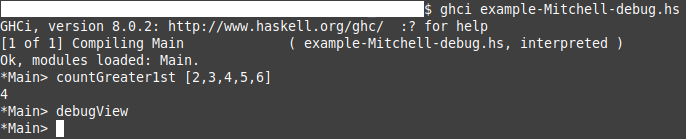
\includegraphics[scale=0.5]{pozivanje-mitchell.png}
\end{center}
Nakon što pozovemo bilo koju funkciju, komandom debugView pozivamo browser prozor koji nam prikazuje željene informacije.
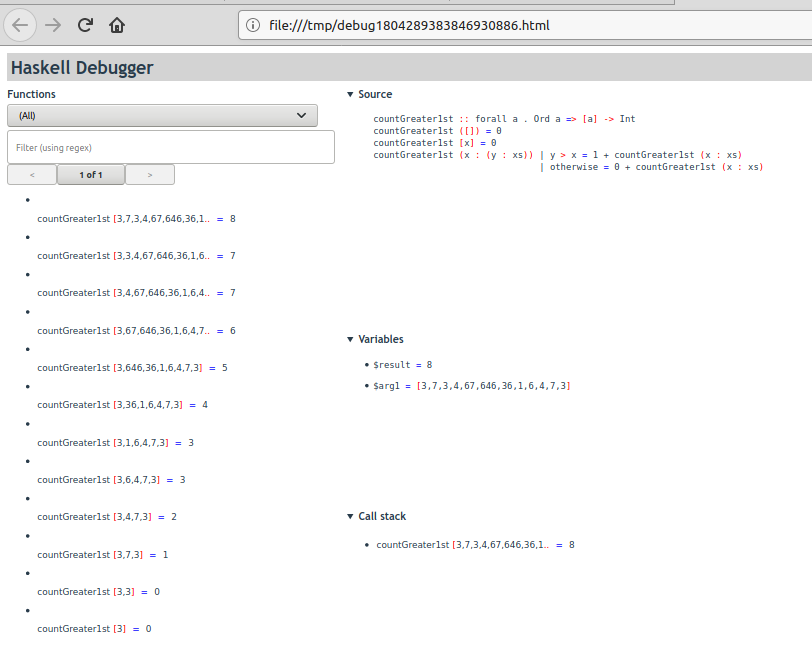
\includegraphics[scale=0.4]{mitchell-browser-pregled.png}
Za svaku od levo navedenih funkcija možemo jasno videti argumente, rezultat i stek, što nam omogućava pregledno debagovanje bilo kog Haskell programa.
Primetićemo da gornji primer radi kako treba. Probajmo sad ostala dva primera.
\end{figure}

\section{Engleski termini i citiranje}	
\label{sec:termini_i_citiranje}

Na svakom mestu u tekstu naglasiti odakle tačno potiču informacije. Uz sve novouvedene termine u zagradi naglasiti od koje engleske reči termin potiče. 

Naredni primeri ilustruju način uvođenja enlegskih termina kao i citiranje.

\begin{primer}
Problem zaustavljanja (eng.~{\em halting problem}) je neodlučiv \cite{haltingproblem}.
\end{primer}

\begin{primer}
Za prevođenje programa napisanih u programskom jeziku C može se koristiti GCC kompajler \cite{gcc}.
\end{primer}

\begin{primer}
 Da bi se ispitivala ispravost softvera, najpre je potrebno precizno definisati njegovo ponašanje \cite{laski2009software}. 
\end{primer}

Reference koje se koriste u ovom tekstu zadate su u datoteci {\em seminarski.bib}. Prevođenje u pdf format u Linux okruženju može se uraditi na sledeći način:
\begin{verbatim}
pdflatex TemaImePrezime.tex 
bibtex TemaImePrezime.aux 
pdflatex TemaImePrezime.tex 
pdflatex TemaImePrezime.tex 
\end{verbatim}
Prvo latexovanje je neophodno da bi se generisao {\em .aux} fajl. {\em bibtex} proizvodi odgovarajući {\em .bbl} fajl koji se koristi za generisanje literature. 
Potrebna su dva prolaza (dva puta pdflatex) da bi se reference ubacile u tekst (tj da ne bi ostali znakovi pitanja umesto referenci). Dodavanjem novih referenci potrebno je ponoviti ceo postupak.  











Broj naslova i podnaslova je proizvoljan. Neophodni su samo Uvod i Zaključak. Na poglavlja unutar teksta referisati se po potrebi. 
\begin{primer}
U odeljku \ref{sec:naslov1} precizirani su osnovni pojmovi, dok su zaključci dati u odeljku \ref{sec:zakljucak}.
\end{primer}

Još jednom da napomenem da nema razloga da pišete:
\begin{verbatim}
\v{s} i \v{c} i \'c ...
\end{verbatim}
Možete koristiti srpska slova
\begin{verbatim}
š i č i ć ... 
\end{verbatim}



\section{Slike i tabele}
\label{slike_i_tabele}

Slike i tabele treba da budu u svom okruženju, sa odgovarajućim naslovima, obeležene labelom da koje omogućava referenciranje. 

\begin{primer} Ovako se ubacuje slika. Obratiti pažnju da je dodato i 
\begin{verbatim}
\usepackage{graphicx}
\end{verbatim}

\begin{figure}[h!]
\begin{center}
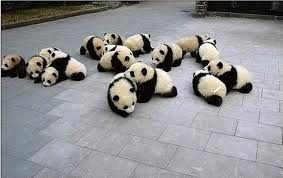
\includegraphics[scale=0.75]{panda.jpg}
\end{center}
\caption{Pande}
\label{fig:pande}
\end{figure}

Na svaku sliku neophodno je referisati se negde u tekstu. Na primer, na slici \ref{fig:pande} prikazane su pande. 
\end{primer}

\begin{primer} I tabele treba da budu u svom okruženju, i na njih je neophodno referisati se u tekstu. Na primer, u tabeli \ref{tab:tabela1} su prikazana različita poravnanja u tabelama.

\begin{table}[h!]
\begin{center}
\caption{Razlčita poravnanja u okviru iste tabele ne treba koristiti jer su nepregledna.}
\begin{tabular}{|c|l|r|} \hline
centralno poravnanje& levo poravnanje& desno poravnanje\\ \hline
a &b&c\\ \hline
d &e&f\\ \hline
\end{tabular}
\label{tab:tabela1}
\end{center}
\end{table}

\end{primer}

\section{K\^{o}d i paket listings}
Za ubacivanje koda koristite paket \textbf{listings}:
\url{https://en.wikibooks.org/wiki/LaTeX/Source_Code_Listings}

\begin{primer}
Primer ubacivanja koda za programski jezik Python dat je kroz listing \ref{simple}. Za neki drugi programski jezik, treba podesiti odgvarajući programski jezik u okviru defnisanja stila.
\end{primer}
\begin{lstlisting}[caption={Primer ubacivanja koda u tekst},frame=single, label=simple]
# This program adds up integers in the command line
import sys
try:
    total = sum(int(arg) for arg in sys.argv[1:])
    print 'sum =', total
except ValueError:
    print 'Please supply integer arguments'
\end{lstlisting}


\section{Prvi naslov}
\label{sec:naslov1}


Ovde pišem tekst. 
Ovde pišem tekst. 
Ovde pišem tekst. 
Ovde pišem tekst. 
Ovde pišem tekst. 
Ovde pišem tekst. 
Ovde pišem tekst. 
Ovde pišem tekst. 


\subsection{Prvi podnaslov}
\label{subsec:podnaslov1}

Ovde pišem tekst. 
Ovde pišem tekst. 
Ovde pišem tekst. 
Ovde pišem tekst. 
Ovde pišem tekst. 
Ovde pišem tekst. 
Ovde pišem tekst. 

\subsection{Drugi podnaslov}
\label{subsec:podnaslov2}

Ovde pišem tekst. 
Ovde pišem tekst. 
Ovde pišem tekst. 
Ovde pišem tekst. 
Ovde pišem tekst. 
Ovde pišem tekst. 


\subsection{... podnaslov}
\label{subsec:podnaslovN}

Ovde pišem tekst. 
Ovde pišem tekst. 
Ovde pišem tekst. 
Ovde pišem tekst. 
Ovde pišem tekst. 
Ovde pišem tekst. 

\section{n-ti naslov}
\label{sec:naslovN}

Ovde pišem tekst. 
Ovde pišem tekst. 
Ovde pišem tekst. 
Ovde pišem tekst. 
Ovde pišem tekst. 

\subsection{... podnaslov}
\label{subsec:podnaslovK}

Ovde pišem tekst. 
Ovde pišem tekst. 
Ovde pišem tekst. 
Ovde pišem tekst. 
Ovde pišem tekst. 

\subsection{... podnaslov}
\label{subsec:podnaslovM}

Ovde pišem tekst. 
Ovde pišem tekst. 
Ovde pišem tekst. 
Ovde pišem tekst. 
Ovde pišem tekst. 


\section{Zaključak}
\label{sec:zakljucak}

Ovde pišem zaključak. 
Ovde pišem zaključak. 
Ovde pišem zaključak. 
Ovde pišem zaključak. 
Ovde pišem zaključak. 
Ovde pišem zaključak. 
Ovde pišem zaključak. 
Ovde pišem zaključak. 
Ovde pišem zaključak. 
Ovde pišem zaključak. 
Ovde pišem zaključak. 
Ovde pišem zaključak. 


\addcontentsline{toc}{section}{Literatura}
\appendix
\bibliography{seminarski} 
\bibliographystyle{plain}

\appendix
\section{Dodatak}
Ovde pišem dodatne stvari, ukoliko za time ima potrebe.
Ovde pišem dodatne stvari, ukoliko za time ima potrebe.
Ovde pišem dodatne stvari, ukoliko za time ima potrebe.
Ovde pišem dodatne stvari, ukoliko za time ima potrebe.
Ovde pišem dodatne stvari, ukoliko za time ima potrebe.


\end{document}
